% Centri — Weekly progress (week ending 2026-08-05)
% Sparse presenting deck (CLAUDE.md rule #5): claim + number + figure + one-line takeaway,
% <=60 words/slide. The cold-readable companion is centri-weekly-2026-08-05-memo.md —
% every claim here appears there with its definition.
% Figures: figs/signfix_*.png, provenance + crops in figs/mk_signfix_figs.py.
% Tables: agent-backend/material_work/_eval/pmagic_tables.{md,tex}, built by
%         agent-backend/tools/build_pmagic_tables.py.
% Compile: pdflatex -interaction=nonstopmode centri-weekly-2026-08-05.tex  (run twice)
\documentclass[aspectratio=169,10pt]{beamer}
\usetheme{metropolis}
\metroset{sectionpage=progressbar, subsectionpage=none, numbering=fraction, progressbar=frametitle}

\usepackage{booktabs}
\usepackage{multirow}
\usepackage{amsmath,amssymb}
\usepackage{xcolor}
\usepackage{colortbl}
\usepackage{graphicx}
\graphicspath{{figs/}}
\usepackage[most]{tcolorbox}

% ---- palette (shared with the other Centri decks) ------------------------
\definecolor{cMeas}{HTML}{1F6FB2}
\definecolor{cPed}{HTML}{B5651D}
\definecolor{cApp}{HTML}{2E7D32}
\definecolor{cInfra}{HTML}{5E35B1}
\definecolor{cAccent}{HTML}{C62828}
\definecolor{cGrey}{HTML}{616161}
\definecolor{cBasic}{HTML}{2E7D32}
\definecolor{cInter}{HTML}{1F6FB2}
\definecolor{cAdv}{HTML}{5E35B1}
\setbeamercolor{frametitle}{bg=cPed}
\setbeamercolor{progress bar}{fg=cAccent}

\newcommand{\ok}{{\color{cApp}\textbf{\checkmark}}}
\newcommand{\nope}{{\color{cGrey}--}}
\newcommand{\takeaway}[1]{\vfill{\footnotesize\itshape\color{cGrey}#1\par}}

% Results tables in P-MAGIC's published layouts (their Tables 2, 3 and 7), generated by
% agent-backend/tools/build_pmagic_tables.py — regenerate, never hand-edit. The deck's word
% budget covers prose only (CLAUDE.md rule #5, revised 2026-07-31): these mirror the published
% tables in full rather than being trimmed to fit a slide.
% Generated by tools/build_pmagic_tables.py — do not edit by hand.
% Layouts mirror Hwang et al. 2026 (refs/document-4.pdf) Tables 2, 3 and 7.

\newcommand{\pmagicCriteria}{%
\begin{tabular}{@{}llp{4.5cm}@{}}
\toprule
\rowcolor{cInfra!12}
\textbf{Dimension} & \textbf{Criterion} & \textbf{Adopted from} \\
\midrule
\textbf{Linguistic / authenticity} & Motivating context & Utami T8 \\
 & Language clarity & Utami T8 / P-MAGIC \\
 & Cognitive demand & Utami T8 \\
 & Fluency & P-MAGIC \\
 & Completeness & P-MAGIC \\
\addlinespace[2pt]
\textbf{Structural / comprehension} & Comprehension & P-MAGIC (ling.\ complexity) \\
 & Structure clarity & Utami T9 \\
 & Concept accuracy & P-MAGIC (concept underst.) \\
 & Realistic & P-MAGIC \\
 & Variable-name consistency & P-MAGIC \\
\addlinespace[2pt]
\textbf{Physics / tier} & Difficulty fit & Centri \\
 & Grounding accuracy & Centri \\
\addlinespace[2pt]
\bottomrule
\end{tabular}}

\newcommand{\pmagicAuto}{%
\begin{tabular}{@{}llcccccccccc@{}}
\toprule
\rowcolor{cMeas!12}
\textbf{Level} & \textbf{n} & \textbf{Stat.} & \textbf{BERT F1} & \textbf{BERT R} & \textbf{BERT P} & \textbf{BLEU-4} & \textbf{ROUGE-1} & \textbf{ROUGE-2} & \textbf{ROUGE-L} & \textbf{Diversity} & \textbf{LSTM} \\
\midrule
basic & 5 & M & 0.799 & 0.790 & 0.808 & 0.019 & 0.270 & 0.038 & 0.132 & 0.185 & n/a \\
 & & SD & 0.002 & 0.004 & 0.002 & 0.008 & 0.017 & 0.007 & 0.008 & --- & n/a \\
\addlinespace[2pt]
intermediate & 5 & M & 0.824 & 0.827 & 0.822 & 0.034 & 0.359 & 0.079 & 0.169 & 0.295 & n/a \\
 & & SD & 0.003 & 0.002 & 0.003 & 0.010 & 0.017 & 0.010 & 0.009 & --- & n/a \\
\addlinespace[2pt]
advanced & 5 & M & 0.828 & 0.828 & 0.828 & 0.035 & 0.404 & 0.095 & 0.176 & 0.316 & n/a \\
 & & SD & 0.003 & 0.004 & 0.002 & 0.010 & 0.014 & 0.009 & 0.007 & --- & n/a \\
\addlinespace[2pt]
\textbf{Total} & 15 & M & 0.817 & 0.815 & 0.819 & 0.029 & 0.344 & 0.071 & 0.159 & 0.293 & n/a \\
 & & SD & 0.013 & 0.018 & 0.009 & 0.012 & 0.058 & 0.026 & 0.021 & --- & n/a \\
\addlinespace[2pt]
\bottomrule
\end{tabular}}

\newcommand{\pmagicMetricDefs}{%
\begin{tabular}{@{}lp{9.4cm}@{}}
\toprule
\rowcolor{cMeas!12}
\textbf{Metric} & \textbf{What it is, and how it is computed} \\
\midrule
\textbf{n} & How many texts the row averages. The unit is one WORKSHEET: n = (clips $\times$ 3 levels), so one third of the Total per level. A per-SECTION figure instead multiplies that by the 5 document sections. The counts printed in the table are computed from the materials actually supplied, never assumed. \\
\textbf{BERT F1} & Meaning overlap. RoBERTa-large turns each word into a context-aware vector and matches it to its closest reference word; F1 is the harmonic mean of R and P below. Raw, not baseline-rescaled, to match P-MAGIC. \\
\textbf{BERT R} & Recall: of the reference's words, how many our text covers. \\
\textbf{BERT P} & Precision: of our words, how many the reference supports. \\
\textbf{BLEU-4} & Exact word-sequence overlap up to 4 words in a row, with a brevity penalty. Near zero for any text that is not a near-copy. \\
\textbf{ROUGE-1} & Single-word overlap with the reference (F1). \\
\textbf{ROUGE-2} & Two-word-sequence overlap (F1). \\
\textbf{ROUGE-L} & Longest common subsequence — shared word order, gaps allowed (F1). \\
\textbf{Diversity} & How much the passages differ from EACH OTHER, not from the reference: one minus their mean pairwise cosine similarity (MiniLM embeddings). Higher means less repetitive. Within a level, and over every worksheet for Total. \\
\textbf{LSTM} & P-MAGIC's fifth metric: a fluency score from an LSTM they trained. Needs their weights, which are unpublished — marked n/a rather than dropped, so the gap stays visible. \\
\bottomrule
\end{tabular}}

\newcommand{\pmagicJudge}{%
\begin{tabular}{@{}l c c cc cc cc @{}}
\toprule
\rowcolor{cPed!12}
& \textbf{Cohen's} & & \multicolumn{2}{c}{\textbf{\color{cBasic}basic}} & \multicolumn{2}{c}{\textbf{\color{cInter}intermediate}} & \multicolumn{2}{c}{\textbf{\color{cAdv}advanced}} \\
\rowcolor{cPed!12}
\textbf{Sub-dimension} & $\boldsymbol{\kappa}$ & \textbf{N} & \textbf{Qwen3.6-35B (local)} & \textbf{Claude Opus 5} & \textbf{Qwen3.6-35B (local)} & \textbf{Claude Opus 5} & \textbf{Qwen3.6-35B (local)} & \textbf{Claude Opus 5} \\
\midrule
\multicolumn{9}{@{}l}{\textbf{Linguistic / authenticity}} \\
\quad Motivating context & -0.04 & 5 & 3.60 \tiny(0.49) & 3.20 \tiny(0.40) & 3.60 \tiny(0.49) & 3.20 \tiny(0.40) & 4.00 \tiny(0.00) & 3.20 \tiny(0.40) \\
\quad Language clarity & 0.19 & 5 & 4.40 \tiny(0.49) & 4.20 \tiny(0.40) & 4.00 \tiny(0.63) & 4.00 \tiny(0.00) & 4.20 \tiny(0.40) & 4.20 \tiny(0.40) \\
\quad Cognitive demand & 0.70 & 5 & 2.80 \tiny(0.40) & 3.00 \tiny(0.00) & 3.60 \tiny(0.49) & 3.20 \tiny(0.40) & 4.80 \tiny(0.40) & 4.20 \tiny(0.40) \\
\quad Fluency & 0.41 & 5 & 4.40 \tiny(0.49) & 3.80 \tiny(0.40) & 4.20 \tiny(0.75) & 3.40 \tiny(0.49) & 4.80 \tiny(0.40) & 4.00 \tiny(0.63) \\
\quad Completeness & 0.58 & 5 & 3.40 \tiny(0.49) & 3.80 \tiny(0.40) & 4.00 \tiny(0.63) & 3.60 \tiny(0.49) & 5.00 \tiny(0.00) & 4.80 \tiny(0.40) \\
\addlinespace[1pt]
\quad\textbf{Linguistic / authenticity --- mean} & 0.52 & 25 & \textbf{3.72} \tiny(0.78) & \textbf{3.60} \tiny(0.57) & \textbf{3.88} \tiny(0.65) & \textbf{3.48} \tiny(0.50) & \textbf{4.56} \tiny(0.50) & \textbf{4.08} \tiny(0.69) \\
\addlinespace[3pt]
\multicolumn{9}{@{}l}{\textbf{Structural / comprehension}} \\
\quad Comprehension & 0.18 & 5 & 4.40 \tiny(0.49) & 3.80 \tiny(0.75) & 4.40 \tiny(0.49) & 3.60 \tiny(0.49) & 4.80 \tiny(0.40) & 4.00 \tiny(0.63) \\
\quad Structure clarity & 0.20 & 5 & 4.40 \tiny(0.49) & 4.00 \tiny(0.00) & 4.40 \tiny(0.49) & 3.60 \tiny(0.49) & 4.80 \tiny(0.40) & 3.80 \tiny(0.75) \\
\quad Concept accuracy & 0.14 & 5 & 2.80 \tiny(0.75) & 3.60 \tiny(0.49) & 3.20 \tiny(1.47) & 3.80 \tiny(0.40) & 4.60 \tiny(0.49) & 4.20 \tiny(0.40) \\
\quad Realistic & 0.29 & 5 & 3.40 \tiny(1.20) & 4.20 \tiny(0.40) & 3.80 \tiny(0.98) & 4.20 \tiny(0.40) & 4.60 \tiny(0.80) & 4.20 \tiny(0.40) \\
\quad Variable-name consistency & 0.51 & 5 & 3.60 \tiny(0.80) & 3.60 \tiny(0.49) & 4.20 \tiny(0.75) & 4.40 \tiny(0.49) & 5.00 \tiny(0.00) & 5.00 \tiny(0.00) \\
\addlinespace[1pt]
\quad\textbf{Structural / comprehension --- mean} & 0.24 & 25 & \textbf{3.72} \tiny(1.00) & \textbf{3.84} \tiny(0.54) & \textbf{4.00} \tiny(1.02) & \textbf{3.92} \tiny(0.56) & \textbf{4.76} \tiny(0.51) & \textbf{4.24} \tiny(0.65) \\
\addlinespace[3pt]
\multicolumn{9}{@{}l}{\textbf{Physics / tier}} \\
\quad Difficulty fit & 0.19 & 5 & 4.20 \tiny(0.40) & 4.20 \tiny(0.40) & 4.00 \tiny(0.89) & 4.20 \tiny(0.40) & 4.40 \tiny(1.20) & 5.00 \tiny(0.00) \\
\quad Grounding accuracy & -0.07 & 5 & 1.40 \tiny(0.49) & 3.20 \tiny(0.75) & 2.60 \tiny(1.96) & 3.40 \tiny(0.80) & 4.00 \tiny(1.26) & 3.60 \tiny(0.49) \\
\addlinespace[1pt]
\quad\textbf{Physics / tier --- mean} & 0.23 & 10 & \textbf{2.80} \tiny(1.47) & \textbf{3.70} \tiny(0.78) & \textbf{3.30} \tiny(1.68) & \textbf{3.80} \tiny(0.75) & \textbf{4.20} \tiny(1.25) & \textbf{4.30} \tiny(0.78) \\
\addlinespace[3pt]
\addlinespace[1pt]
\textbf{All 12 criteria} & 0.31 & 60 & \textbf{3.57} \tiny(1.07) & \textbf{3.72} \tiny(0.61) & \textbf{3.83} \tiny(1.07) & \textbf{3.72} \tiny(0.61) & \textbf{4.58} \tiny(0.71) & \textbf{4.18} \tiny(0.70) \\
\addlinespace[3pt]
\bottomrule
\end{tabular}}



\title{Centri --- Scoring the Material}
\subtitle{One rubric for the model and the teachers --- see the accompanying memo for detail}
\author{Damar Albaribin}
\institute{MSc Thesis --- advisor: Prof.\ Wu-Yuin Hwang}
\date{Week ending 2026-08-05}

\begin{document}
\maketitle

% =========================================================================
\begin{frame}{Where the work stands}
\vfill
\begin{center}
{\Large One phone video $\rightarrow$ \textbf{\color{cBasic}basic} $\cdot$
\textbf{\color{cInter}intermediate} $\cdot$ \textbf{\color{cAdv}advanced}}\\[3pt]
{\footnotesize 7 clips, 21 worksheets}
\end{center}
\vfill
\begin{center}
\small
\renewcommand{\arraystretch}{1.6}
\begin{tabular}{@{}p{7.4cm}c@{}}
\toprule
\rowcolor{cPed!12}
\textbf{Question} & \\
\midrule
Do the numbers trace to the measurement? & \ok \\
\textbf{Is the measurement itself right?} & {\color{cAccent}\textbf{6 of 7 clips}} \\
Does it get harder by level? & \ok \\
Do the figures agree with the text? & {\color{cAccent}\textbf{4 defects open}} \\
\textbf{Does anybody learn from it?} & {\color{cAccent}\textbf{?}} \\
\bottomrule
\end{tabular}
\end{center}
\vfill
\takeaway{Tracing a number to the measurement is not the same as the measurement being right ---
one clip's is not. The last row is the question the project is actually asking.}
\end{frame}

% =========================================================================
\begin{frame}{A graph that argued with its own caption}
\vfill
\begin{columns}[T,onlytextwidth]
\begin{column}{0.5\textwidth}
\begin{center}
{\footnotesize\color{cAccent}\textbf{shipped}}\\[2pt]
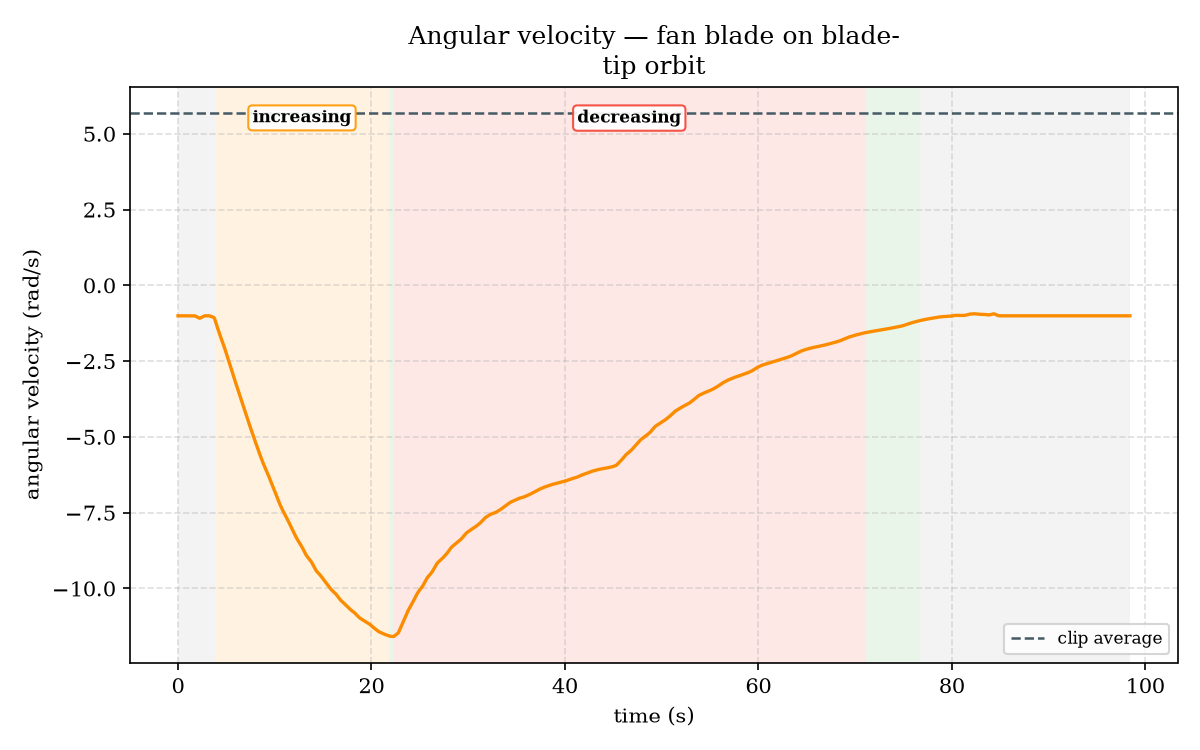
\includegraphics[width=\linewidth]{signfix_omega_before.png}
\end{center}
\end{column}
\begin{column}{0.5\textwidth}
\begin{center}
{\footnotesize\color{cApp}\textbf{now}}\\[2pt]
\includegraphics[width=\linewidth]{signfix_omega_after.png}
\end{center}
\end{column}
\end{columns}
\vfill
\begin{center}
{\footnotesize The dashed ``clip average'' sat at $+5.7$, above every point on the curve.
The band marked \emph{increasing} is where the line falls. {\color{cAccent}That dashed line is
\emph{still} mislabelled} --- it averages the turning part only.}
\end{center}
\takeaway{The camera decides the sign, not the physics. A reader needs the speed.}
\end{frame}

% =========================================================================
\begin{frame}{The arrows pointed the wrong way}
\vfill
\begin{columns}[T,onlytextwidth]
\begin{column}{0.5\textwidth}
\begin{center}
{\footnotesize\color{cAccent}\textbf{shipped}}\\[2pt]
\includegraphics[width=\linewidth]{signfix_arrows_before_crop.png}
\end{center}
\end{column}
\begin{column}{0.5\textwidth}
\begin{center}
{\footnotesize\color{cApp}\textbf{now}}\\[2pt]
\includegraphics[width=\linewidth]{signfix_arrows_after_crop.png}
\end{center}
\end{column}
\end{columns}
\vfill
\begin{center}
{\footnotesize Both ceiling fans turn counter-clockwise. Every one of their six worksheets
drew $v$ and $\omega$ backwards.}
\end{center}
\takeaway{Caused by the previous fix: once the stored value became a magnitude, the code
asking it for a direction always got ``clockwise''.}
\end{frame}

% =========================================================================
\begin{frame}{The tracker jumps}
\vfill
\begin{center}
\includegraphics[width=0.66\textwidth]{jump_tt3.png}
\end{center}
\begin{center}
{\footnotesize The marker normally moves $1.4$~px between frames. Three times it moves
$604$--$713$~px in one. One of the three is inside the measured window.}
\end{center}
\takeaway{The worksheet teaches an inward pull of \textbf{7.45}~m/s$^2$. Without the jumps it is
\textbf{5.85} --- $27\%$ too high.}
\end{frame}

% =========================================================================
\begin{frame}{How far it spreads}
\vfill
\begin{center}
\small
\renewcommand{\arraystretch}{1.35}
\begin{tabular}{@{}lccc@{}}
\toprule
\rowcolor{cAccent!10}
\textbf{Clip} & \textbf{jumps} & \textbf{in the measured window} & \textbf{taught numbers} \\
\midrule
turntable-3 & 3 & {\color{cAccent}\textbf{1}} & {\color{cAccent}\textbf{wrong by 27\%}} \\
computerfan-4029 & 4 & 0 & unaffected \\
\midrule
fan-4027 $\cdot$ fan-4028 & 0 & --- & unaffected \\
roundabout-4046 & 0 & --- & unaffected \\
turntable-1 $\cdot$ turntable-2 & 0 & --- & unaffected \\
\bottomrule
\end{tabular}
\end{center}
\vfill
\begin{center}
{\footnotesize Detected per clip against its \emph{own} normal step --- a fixed threshold would
condemn the fan, which really does travel $240$~px between frames.}
\end{center}
\takeaway{Five of seven are clean. One clip's published numbers are wrong, and it took a
question about a graph to find it.}
\end{frame}

% =========================================================================
\begin{frame}{Automatic evaluation, by level}
\vfill
\begin{center}
% 12 columns overrun the slide at any readable point size — scale to the text width rather
% than dropping a metric. \resizebox needs the tabular as its sole argument.
\scriptsize
\renewcommand{\arraystretch}{1.15}
\resizebox{\textwidth}{!}{\pmagicAuto}
\end{center}
\vfill
\begin{center}
{\scriptsize P-MAGIC Table 3 layout (their Easy / Intermediate / Advanced), where BERT F1 runs
$0.877$--$0.885$ and diversity $\approx 0.51$. Each column is defined overleaf.}
\end{center}
\takeaway{Every column rises with the level. Spread \emph{within} a level is $\pm 0.003$, across
all 21 it is $\pm 0.014$ --- these are reading the level, not the video.}
\end{frame}

% =========================================================================
\begin{frame}{What each score measures}
\begin{center}
\scriptsize
\renewcommand{\arraystretch}{1.0}
\pmagicMetricDefs
\end{center}
\takeaway{Higher means ``more like OpenStax'' --- not ``teaches better''.}
\end{frame}

% =========================================================================
\begin{frame}{The instrument}
\begin{center}
\scriptsize
\renewcommand{\arraystretch}{1.05}
\pmagicCriteria
\end{center}
\begin{center}
{\scriptsize Twelve \emph{text} criteria, each scored \textbf{1--5}. Ten adopted from the parent
line so the rows line up with theirs; two are Centri's. \textbf{A further eleven score the
figures} (Axis 4, overleaf) --- 23 in all.}
\end{center}
\takeaway{The same instrument goes to the teachers, unchanged. Only the rater differs.}
\end{frame}

% =========================================================================
\begin{frame}{LLM-judge results, every criterion}
\begin{center}
\tiny
\renewcommand{\arraystretch}{0.98}
\pmagicJudge
\end{center}
\begin{center}
{\scriptsize Two \textbf{LLM} raters, same 21 worksheets: local \texttt{Qwen3.6-35B} and
\texttt{Claude Opus 5}. \textbf{Cohen's $\kappa$}, quadratic-weighted, is \textbf{model-vs-model}
--- P-MAGIC's $0.76$ is human-vs-human. $N$ = ratings per mean. \emph{Continued overleaf.}}
\end{center}
\takeaway{Both raters put advanced top. Neither agrees with the other on what the score is:
$\kappa = 0.34$ overall.}
\end{frame}

% =========================================================================
\begin{frame}{LLM-judge results, the figures}
\begin{center}
\scriptsize
\renewcommand{\arraystretch}{0.95}
\pmagicJudgeMM
\end{center}
\begin{center}
{\scriptsize Same table, same columns --- Axis 4. Scored by the \textbf{vision} rater only.
A dash at basic = the tier \textbf{prints no table by design}.}
\end{center}
\takeaway{Our own row --- the annotated frame --- is the strongest here; the figures do not get
harder by level.}
\end{frame}

% =========================================================================
\begin{frame}{Two judges, one rubric}
\vfill
\begin{center}
\small
\renewcommand{\arraystretch}{1.2}
\begin{tabular}{@{}lccc@{}}
\toprule
\rowcolor{cPed!12}
\textbf{Level} & \textbf{Qwen3.6-35B} & \textbf{Claude Opus 5} & \textbf{gap} \\
\midrule
basic        & 3.99 & 3.45 & $-0.54$ \\
intermediate & 3.92 & 3.43 & $-0.49$ \\
advanced     & \textbf{4.46} & \textbf{3.96} & $-0.50$ \\
\addlinespace[2pt]
\midrule
\multicolumn{4}{@{}l}{\textbf{Where they agree, and where they do not}} \\
Cognitive demand \ {\footnotesize\color{cGrey}the tier ladder} &
  \multicolumn{3}{c}{$\kappa = {\color{cApp}\mathbf{0.59}}$} \\
Grounding accuracy \ {\footnotesize\color{cGrey}whether the numbers hold up} &
  \multicolumn{3}{c}{$\kappa = {\color{cAccent}\mathbf{-0.04}}$} \\
\bottomrule
\end{tabular}
\end{center}
\vfill
\begin{center}
{\scriptsize 252 paired ratings. Same score 33\% of the time, within one point 88\%.\\
On \texttt{turntable-3}'s advanced worksheet --- the one whose numbers \emph{are} wrong ---
Qwen scored grounding \textbf{5}, Claude \textbf{2}.\\
Not noise: re-run two days on, the local judge repeated all 252 ratings exactly.}
\end{center}
\takeaway{The ranking reproduces across raters; the score does not.}
\end{frame}

% =========================================================================
\begin{frame}{A caption that denied its own curve}
\begin{center}
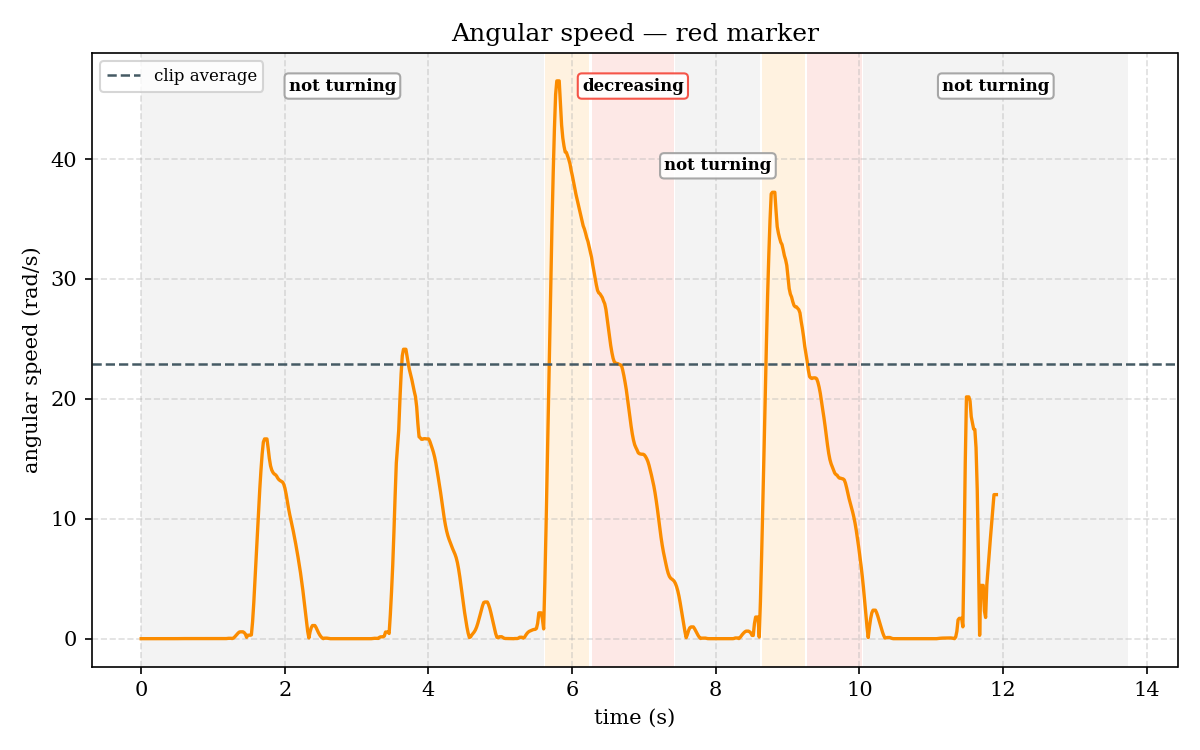
\includegraphics[width=0.60\textwidth]{notturning_before.png}
\end{center}
\begin{center}
{\scriptsize Three bands captioned \textbf{``not turning''}, over samples reaching
\textbf{24 rad/s}. The segmenter marks bursts as rest; printing the word made a silent error into
a stated claim. \textbf{11 of the corpus's 12} rest bands read like this.\\
Now suppressed wherever the curve disagrees --- {\color{cAccent}the boundaries themselves are
still wrong}.}
\end{center}
\takeaway{The checker passed it --- it never asks whether a caption agrees with its curve.}
\end{frame}

% =========================================================================
\begin{frame}{Where each rater was right}
\vfill
\begin{center}
\small
\renewcommand{\arraystretch}{1.5}
\begin{tabular}{@{}p{5.4cm}p{6.0cm}@{}}
\toprule
\rowcolor{cPed!12}
\textbf{The LLM judge said} & \textbf{Verdict} \\
\midrule
$8.04^2 \times 0.438 = 28.3$ is wrong & {\color{cAccent}\textbf{the judge was wrong}}
--- right to 3 figures \\
turntable-3's inward pull of $7.45$ is not grounded &
{\color{cApp}\textbf{the judge was right}} --- it is a tracker artifact, truly $5.85$ \\
\bottomrule
\end{tabular}
\end{center}
\vfill
\begin{center}
{\footnotesize The machine checker passed $7.45$ because it \emph{does} trace to the
measurement. It cannot ask whether the measurement is sound.}
\end{center}
\takeaway{Tracing a number is not validating it --- and the model caught what the checker,
by construction, never could.}
\end{frame}

% =========================================================================
\begin{frame}{One rubric, two kinds of rater}
\vfill
\begin{center}
\small
\renewcommand{\arraystretch}{1.5}
\begin{tabular}{@{}p{4.9cm}ccc@{}}
\toprule
\rowcolor{cInfra!12}
& \textbf{Qwen3.6-35B} & \textbf{Claude Opus 5} & \textbf{teachers} \\
\midrule
same 12 criteria, same 1--5 scale & \ok & \ok & \ok \\
scores all 21 worksheets & \ok & \ok & \ok \\
\midrule
independent of the writer & \nope & \ok & \ok \\
can say whether it \emph{teaches} & \nope & \nope & \ok \\
\bottomrule
\end{tabular}
\end{center}
\vfill
\begin{center}
{\footnotesize \texttt{Qwen3.6-35B} also \emph{wrote} the material, so it grades its own work ---
which is why the second rater is from a different family. P-MAGIC scored 10-point; ours is 1--5.}
\end{center}
\takeaway{The instrument runs, and now with two raters. Neither can say whether anyone learns.}
\end{frame}

% =========================================================================
\begin{frame}{Checks a model never sees}
\vfill
\begin{center}
\small
\renewcommand{\arraystretch}{1.45}
\begin{tabular}{@{}p{6.8cm}c@{}}
\toprule
\rowcolor{cApp!12}
\textbf{Machine checker, 21 worksheets} & \textbf{clean} \\
\midrule
arithmetic, grounding, tier rules, wording & 19 / 21 \\
\quad{\footnotesize plus the new same-moment rule} & \textbf{13 / 21} \\
\bottomrule
\end{tabular}
\end{center}
\vfill
\begin{center}
{\footnotesize ``a lap of 2.07~s \dots\ \emph{that} rate, 0.30 turns each second''
--- which is a 3.34~s lap. Six worksheets, all beginner.}
\end{center}
\takeaway{It agrees with the LLM judge clip for clip: the same six flagged, the same one clean.
Two raters, no shared code.}
\end{frame}

% =========================================================================
\begin{frame}{Bahasa Indonesia edition}
\vfill
\begin{center}
{\Large \textbf{42} documents --- 7 clips $\times$ 3 levels $\times$ student and teacher}
\end{center}
\vfill
\begin{center}
\small
\renewcommand{\arraystretch}{1.4}
\begin{tabular}{@{}p{5.2cm}p{5.6cm}@{}}
\toprule
\rowcolor{cInfra!12}
\textbf{Choice} & \textbf{Why} \\
\midrule
translate the finished page & only 17--32\% of it is prose \\
verify every number after & a translation must not move a digit \\
one fixed glossary & terms stay steady across levels \\
decimals stay \texttt{0.26} & keeps the number check valid \\
\bottomrule
\end{tabular}
\end{center}
\vfill
\takeaway{Built for the teacher panel, which will read in Bahasa Indonesia.}
\end{frame}

% =========================================================================
\begin{frame}{What is still unproven}
\vfill
\begin{center}
\small
\renewcommand{\arraystretch}{1.6}
\begin{tabular}{@{}p{5.4cm}p{5.6cm}@{}}
\toprule
\rowcolor{cAccent!10}
\textbf{Measured} & \textbf{Not measured} \\
\midrule
the numbers are right & anybody understands them \\
the levels differ & the levels differ \emph{for a learner} \\
the reader is asked to act & the reader acts \\
\midrule
\multicolumn{2}{@{}l}{{\footnotesize P-MAGIC: ten teachers, 8.2--8.6 / 10.\quad
Centri: one expert reader, two models.}} \\
\bottomrule
\end{tabular}
\end{center}
\vfill
\takeaway{Teacher ratings are the next step --- after repairing the one criterion the two judges
cannot agree on. Teachers would inherit the same ambiguity.}
\end{frame}

\end{document}
